\documentclass[journal,twoside]{JoPhA}

\usepackage{flushend}
\usepackage{color}
\usepackage{graphicx}

\begin{document}

\title{Strategies for Haptic-Robotic Teleoperation in Board Games: Playing checkers with Baxter}

\author{Francisco J. Rodr\'{i}guez--Sedano, Gonzalo Esteban, Laura Inyesto, Pablo Blanco, Francisco J. Rodr\'{i}guez--Lera

\IEEEcompsocitemizethanks{\IEEEcompsocthanksitem Robotics Group. University of Le\'{o}n.\protect\\

E-mail: francisco.sedano@unileon.es, gestc@unileon.es, linyea00@estudiantes.unileon.es, pblanm02@estudiantes.unileon.es, fjrodl@unileon.es}
}


\markboth{Journal of Physical Agents,~Vol.~1, No.~1, July~2007}%
{Cazorla and Matellan : JoPhA Paper Demo}
\maketitle


\begin{abstract}
Teleoperating robots is quite a common practice in fields such as surgery, defence or rescue. The main source of information in this kind of environments is the sense of sight. The user can see on a display what the robot is watching in real time, and maybe also a visual representation of the robot surroundings. Our proposal involves the use of haptic devices to teleoperate a robot, Baxter, in order for the user to obtain haptic feedback besides visual information. As a proof of concept, the proposed environment is checkers playing. Our goal is testing if the inclusion of the sense of touch improves the user experience or not. 
\end{abstract}


\begin{IEEEkeywords}
JoPhA, journal, \LaTeX, paper, template.
\end{IEEEkeywords}


\section{Introduction}
% GONZALO

% Teleoperation-telemanipulation and user experience
  \IEEEPARstart{T}{eleoperating} robots is quite a common practice in many fields such as surgery, defence or rescue~\cite{Vertut85}. The reason is simple: assisting a person to perform and accomplish complex or uncertain tasks in some environments may mean the difference between failure or success.

  Enhancing the user experience is a key aspect in teleoperation. These systems use different interfaces (e.g. cameras, microphones or input devices) to provide sensory information to the operator, and thus, improving the user experience. Traditionally, video feedback from an on-board or front-mounted camera is limited by technical constraints~\cite{Woods04,Woods97} like a restricted field of view or poor resolution. In some scenarios, these constraints makes difficult for the operator to be aware of the robot's proximity to objects~\cite{Alfano90}, causing a decrease in performance. To alleviate such limitations, at least partially, haptic cues (either by force or tactile feedback) have been shown to be useful in some applications~\cite{Son13,Sitti03,Diolaiti02}, especially when the operator performs manipulation tasks~\cite{King09,Kron04}.
  
  Haptic feedback is very important when simulating interactions with rigid objects. When interacting with rigid objects like exploring the edges, surfaces features, etc. visual information is replaced by the sense of touch.  % add some brief literature review about haptics in teleoperation

  % TELEMANIPULATION SYSTEMS AND BILATERAL TELEOPERATION. Highlight bilateral teleoperation using position [Kuchenbecker 2006].
  
  
% GOALS OF THE PAPER
  The motivation behind this paper is to test whether or not the sense of touch improves the user experience in teleoperation. To achieve this, we propose an experiment: teleoperate a robot for playing a board game. The scenario will have two players and one game. One player is located at the game's place while the other is away, teleoperating a robot which is ``physically'' located at that same place. The teleoperation system consists of a Geomagic Touch haptic interface (that acts as a master device) and a Baxter robot (which acts as the slave device). The board game chosen to play is ``checkers'', a strategy game chosen because of its simplicity: all pieces are equal except from their colors and they can only move diagonally forward. With this setup, the user experience is evaluated by defining and measuring some metrics with a group of expert's evaluators.

% STRUCTURE
  This paper is organized as follows. Section~\ref{sec:environment} shows the architecture of the environment by describing the basic elements of the system. Section~\ref{sec:experiment} describes how the experiment has been defined and carried out. Finally, the paper ends with our conclusions.

\section{Environment description}
\label{sec:environment}

  Any telemanipulation system is comprised of two robots, master and slave, and a communication channel that physically links them. The master allows an operator to send commands to control the slave motion, while the slave robot interacts with the environment by executing such commands. Since the goal of this paper is to test if haptic feedback improves the user experience, the master robot must be a haptic device. To play a board game, the slave robot must be placed in a fixed location and be able to grasp and manipulate objects with precision. Our system is comprised of a Geomagic Touch haptic device and a Baxter robot acting as master and slave, respectively.
    
  To perform the experiment, the environment needs to be a place where a board game can be played. The game mechanics must be as simple as posible, so that the user focuses on the manipulation aspects, i.e. grasping the game pieces and moving them along the board. Because Baxter needs a large workspace the game board needs to be big enough; as well as the game pieces, in order to be easily grasped by the robot's end effector. After considering several options ``Checkers'' was selected.
  
  So the choosen environment is a room containing two separated tables: one for the Checkers board and one for the operator (see figure~\ref{fig:environment:environment}). The game's table contains the Checkers board and pieces. The operator's table contains the master device and a workstation. To ignore the communication channel time delays both, master and slave, are connected to such workstation through Ethernet cables.
    
%GONZALO: SHOULD WE ADD THIS PIC TO ILLUSTRATE THE ENVIRONMENT¿?
\begin{figure}[!ht]
  \centering
  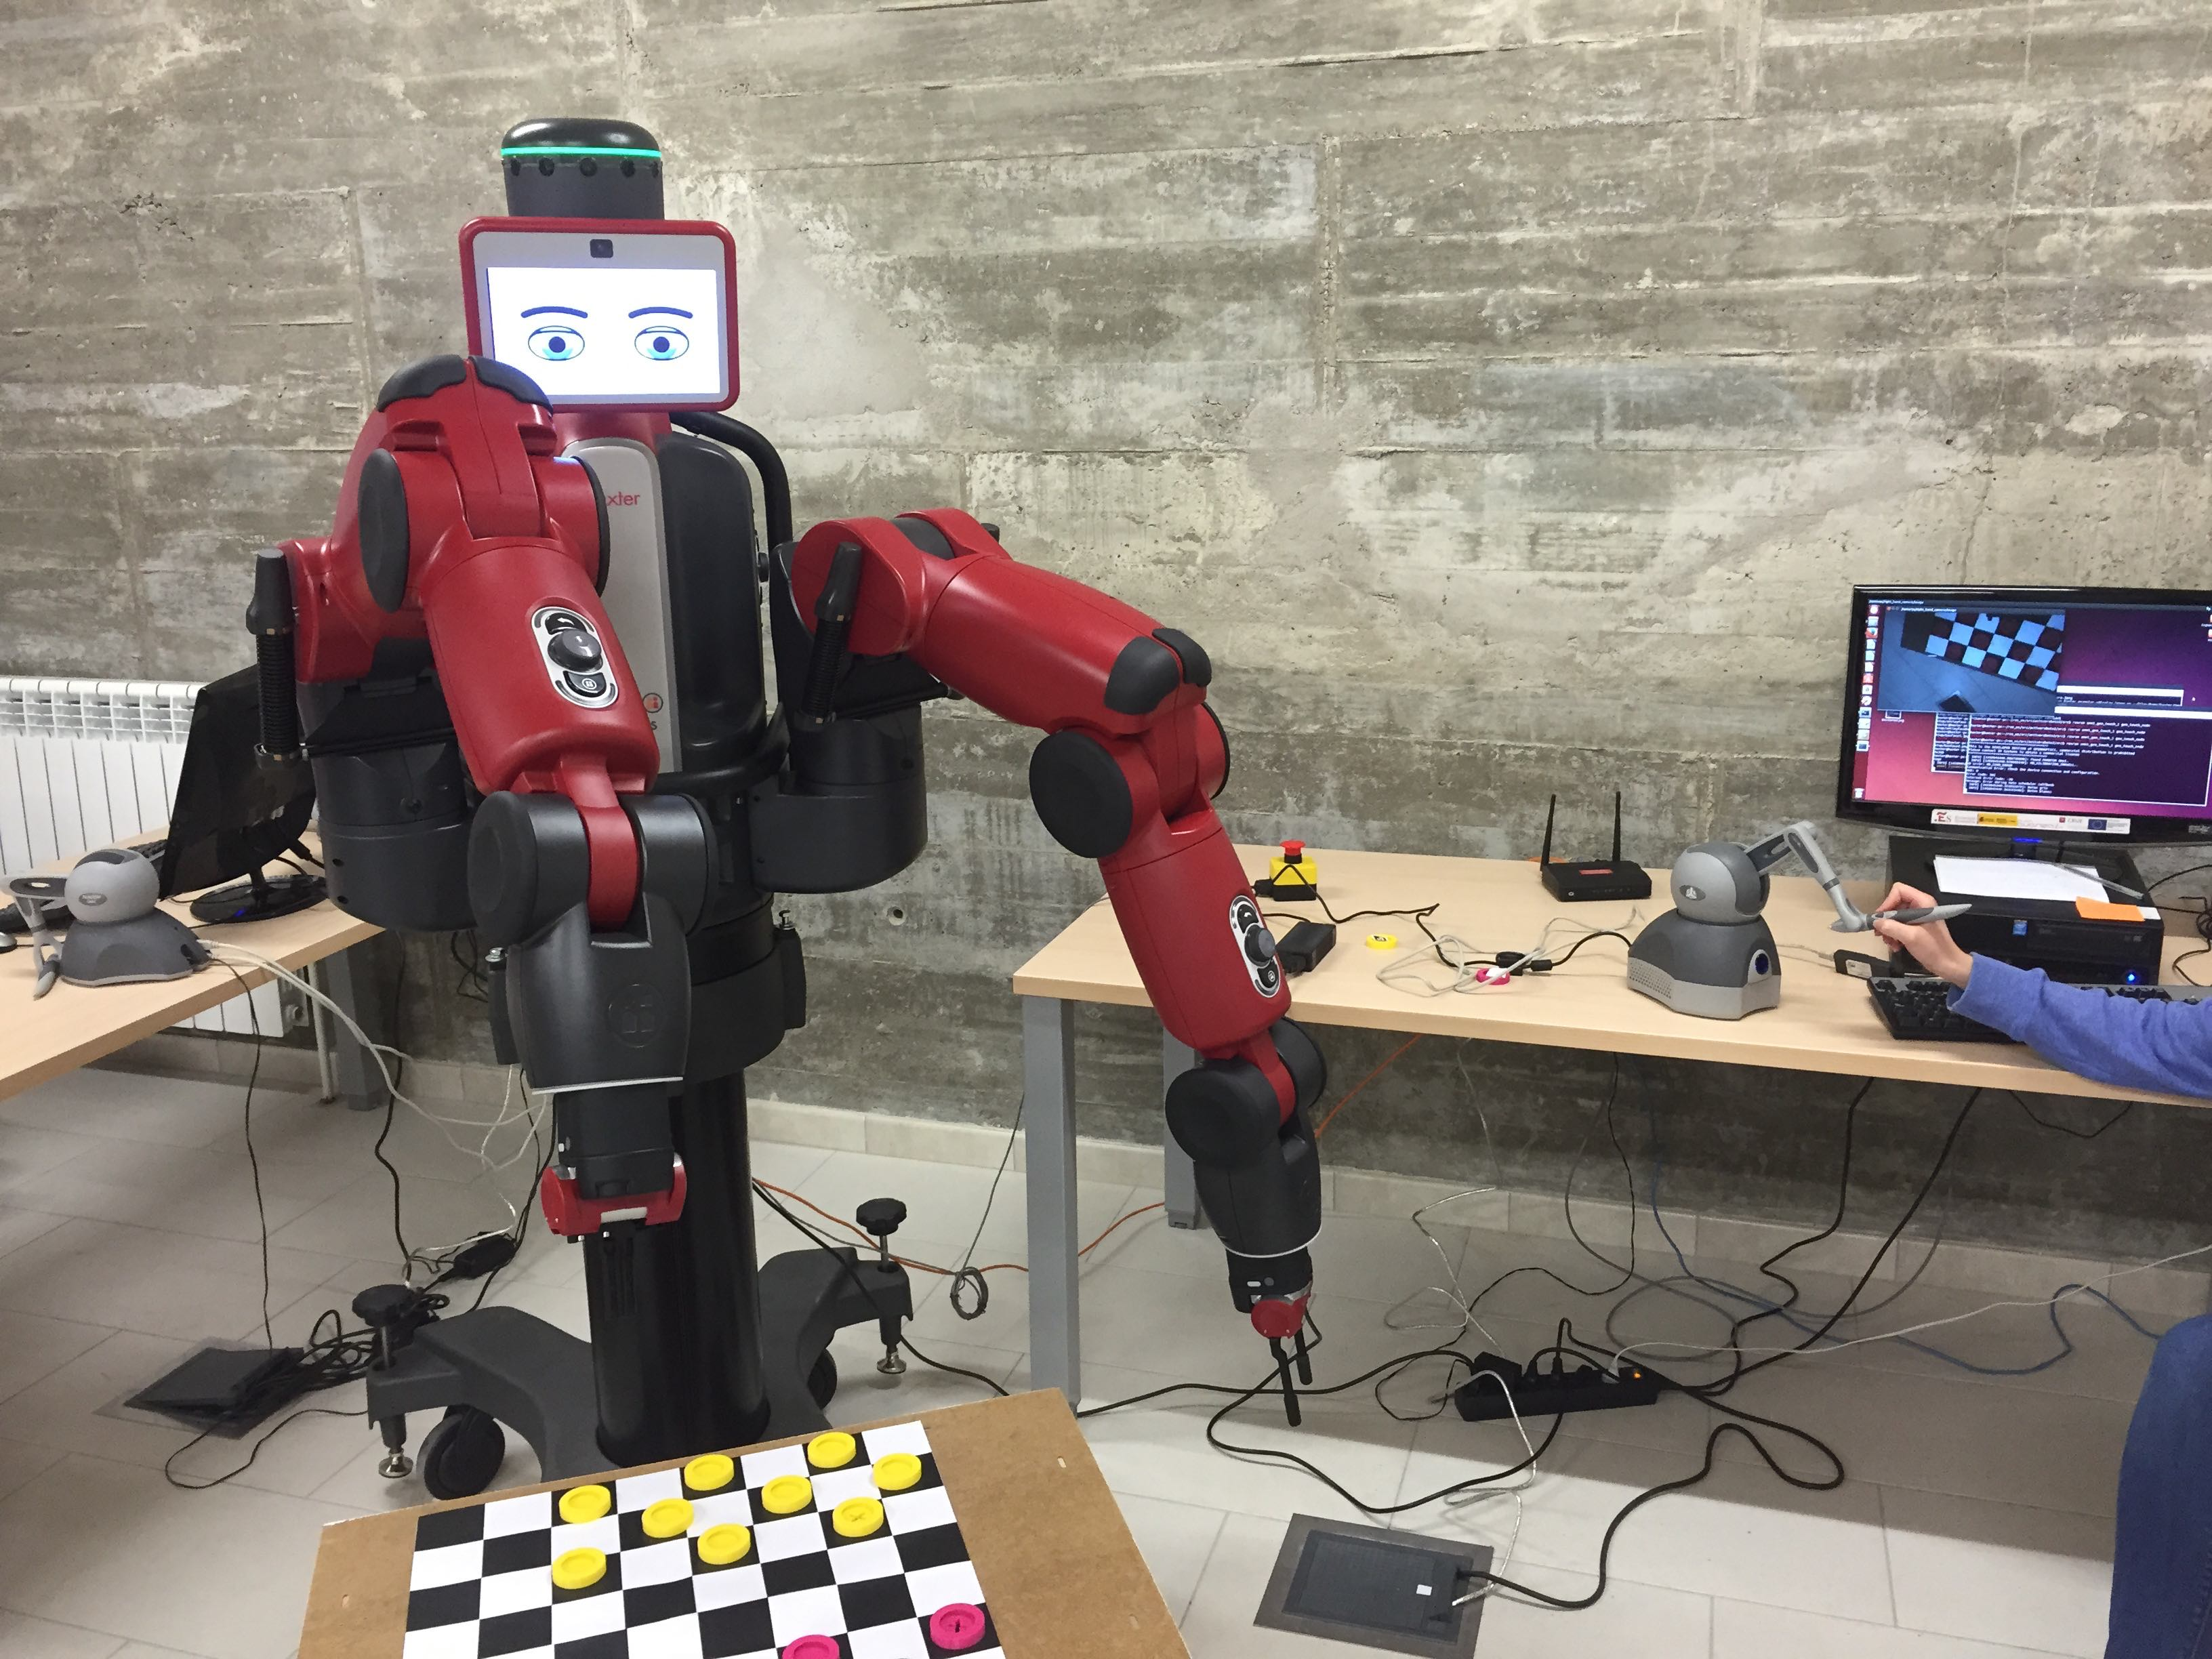
\includegraphics[width=0.45\textwidth]{Images/Baxter&Haptic.jpg}
  
  \caption{Environment used for the experiment.}
  \label{fig:environment:environment}
\end{figure}

  \subsection{Master: Geomagic Touch}
  \label{sec:environment:master}

%GONZALO: I think we should remove this paragraph because this is explained in the introduction.
%  Haptic feedback takes advantage of the human sense of touch by recreating forces, vibrations   or motions to the user. A haptic device allows to feel a feedback from virtual or real objects and produces a realistic touch sensations to a user. 

  The master device needs to be able to send the operator's movements and commands to Baxter, but at the same time, provide some kinesthetic information to the operator, i.e. reflect the forces or vibrations sensed by Baxter. In the experiment's context, haptic devices capable of force feedback perfectly fits as a master device; particularly, we used a Geomagic Touch haptic device (see figure~\ref{fig:environment:master}).
    
\begin{figure}[!ht]
  \centering
  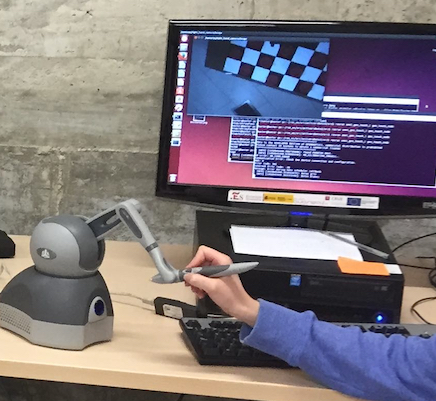
\includegraphics[scale=0.5]{Images/BaxterYHapticSmall.jpg}
  
  \caption{Geomagic Touch haptic device.}
  \label{fig:environment:master}
\end{figure}

  The Geomagic Touch is a 6 DOF device, that has 3 actuated DOF associated to the armature which provides the translational movements (X, Y, and Z Cartesian coordinates) and other 3 non-actuated DOF associated to the gimball that gives the orientation (pitch, roll and yaw rotational movements). Also, the device is able to perform a force up to a maximum of 3.3~N within a workspace of 160 (width) $\times$ 120 (height) $\times$ 70 (depth)~mm. These characteristics are more than enough to both, translate the operator's movement using the device's stylus and feel the environment perceived by Baxter using the device's actuators.
  
  The device is connected to a workstation running Ubuntu 14.04 (Trusty) with ROS Indigo. To communicate the haptic device with ROS, we used the package ``\emph{phantom-{}omni}'' developed by Suarez-Ruiz~\cite{SuarezRuiz12}. However, this package was developed for ROS Hydro, so we adapted it and developed a new teleoperator program to control Baxter.

  \subsection{Slave: Baxter}
  \label{subsec:environment:slave}

  The slave device needs to mimic the operator's movement and be able to grab or translate the Checker's pieces. For the experiment we used a Baxter robot (see figure~\ref{fig:environment:slave}).

\begin{figure}[!ht]
  \centering
  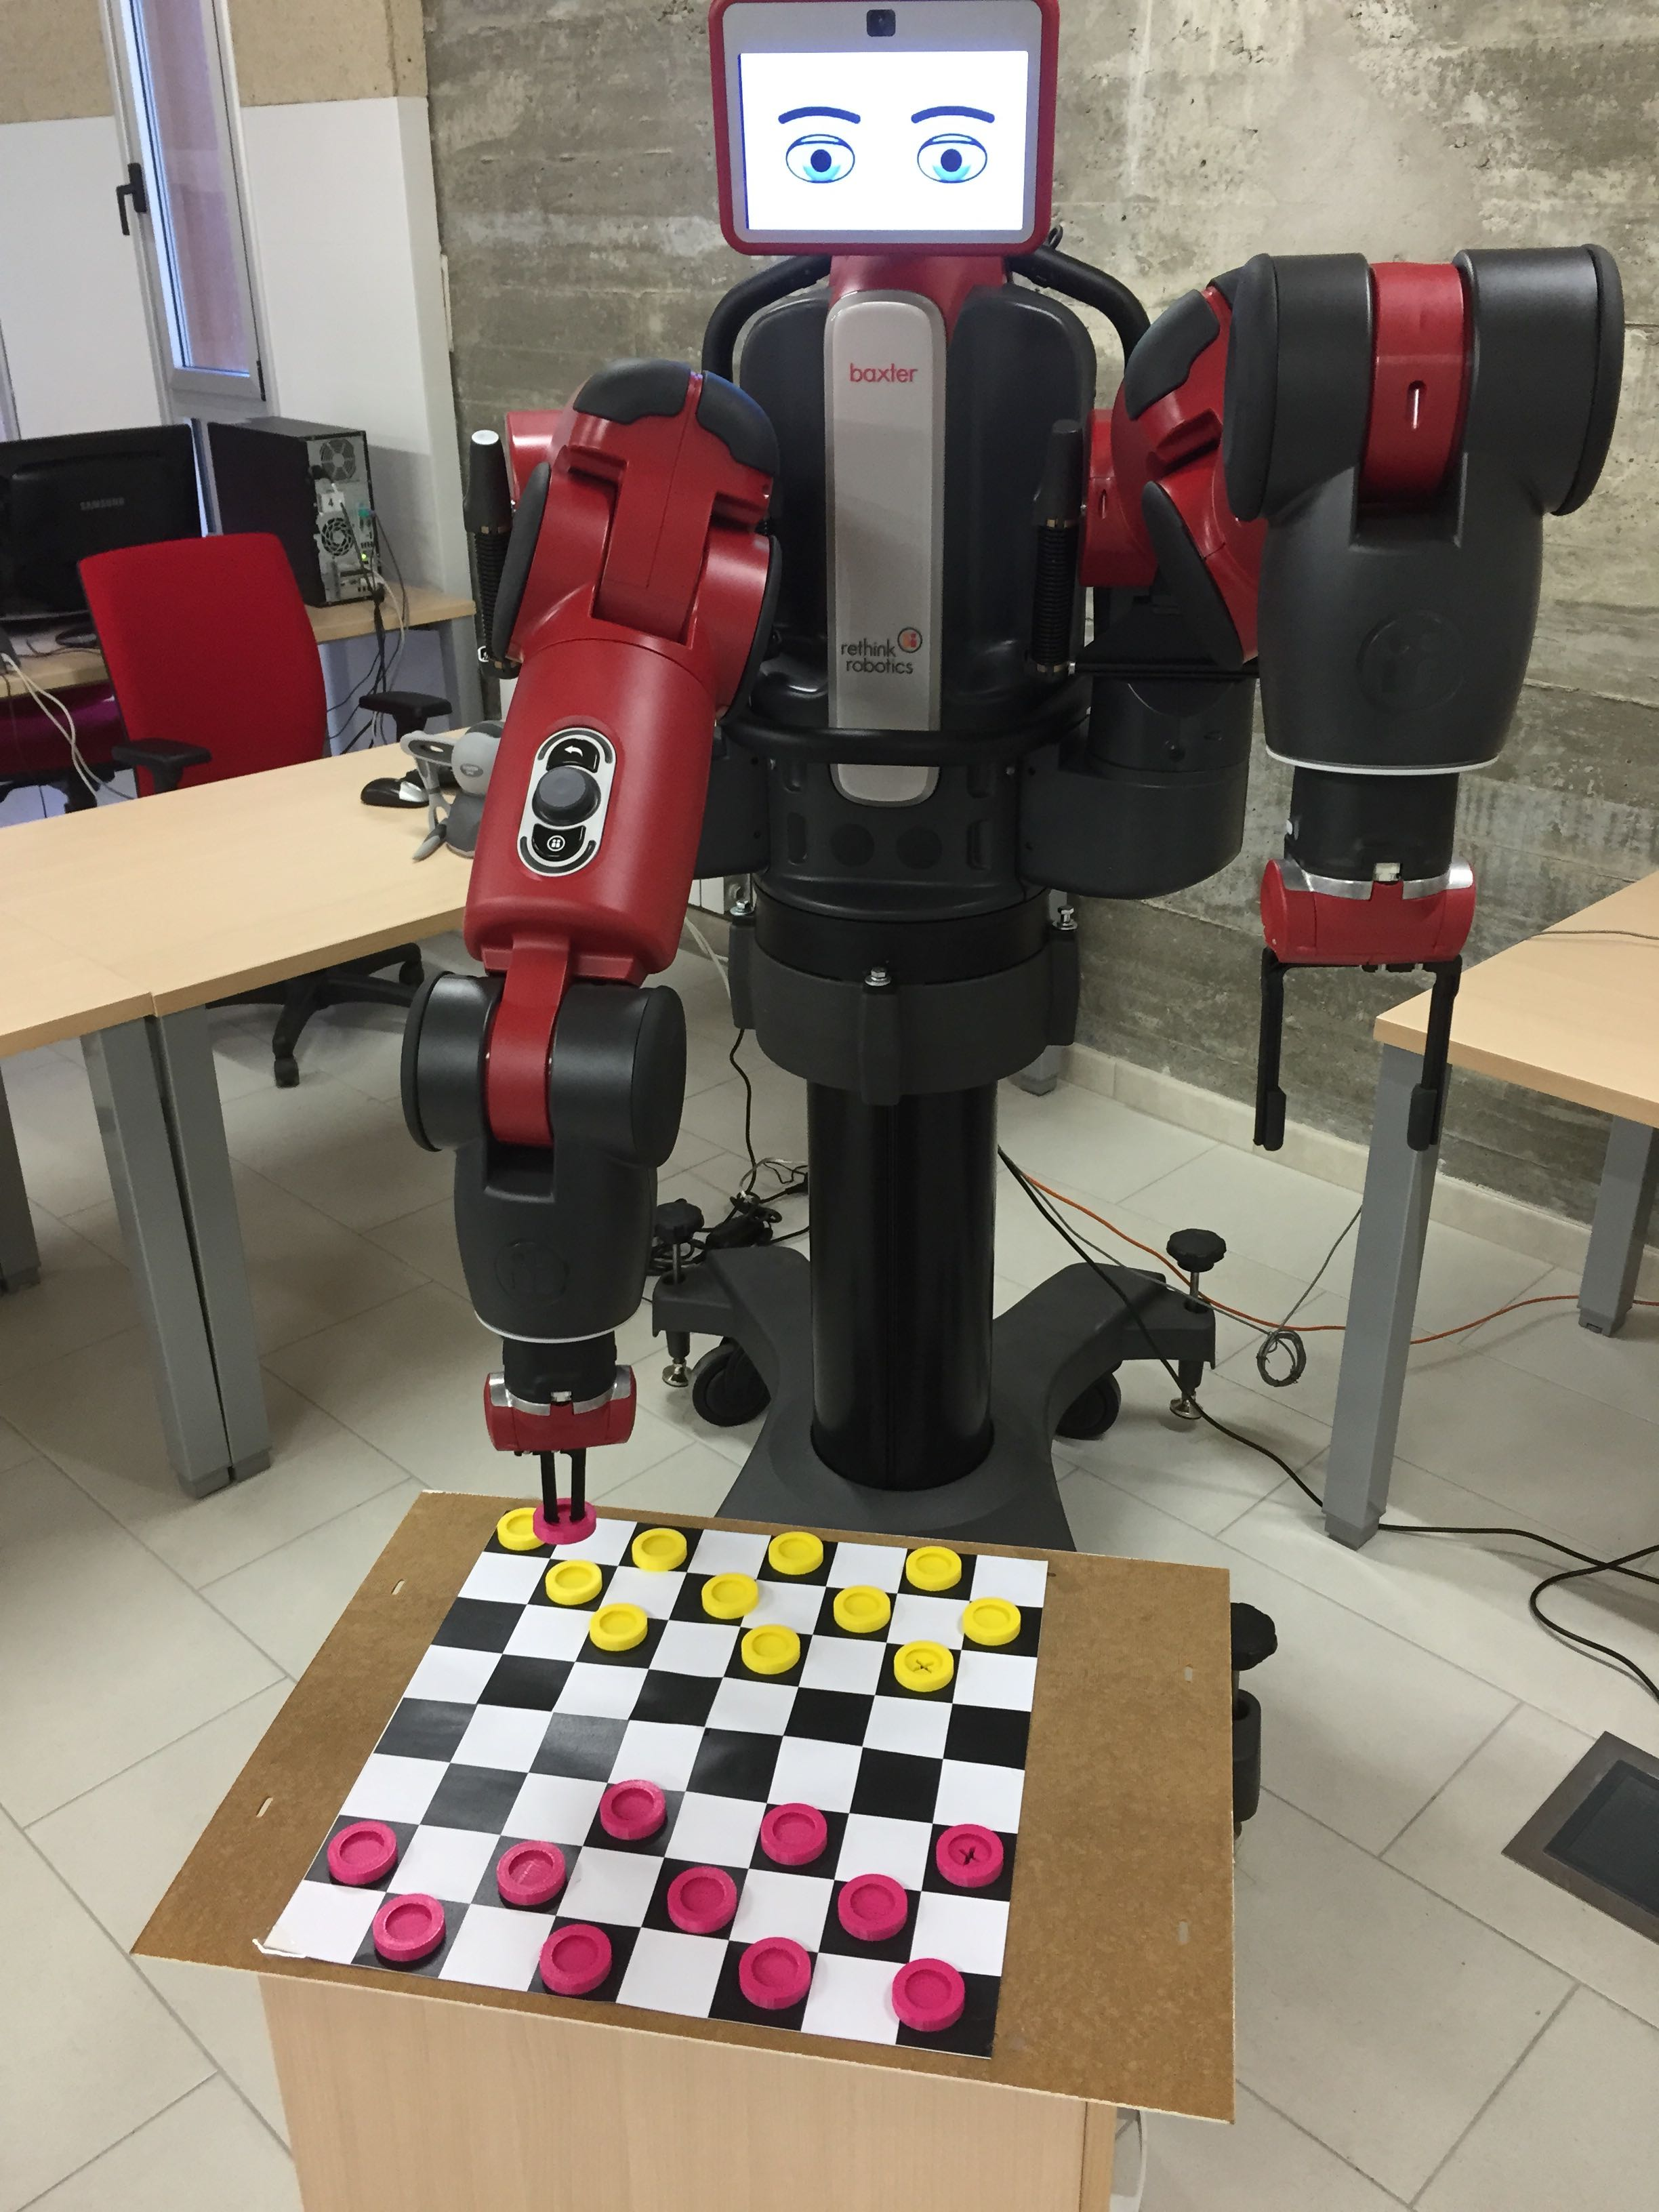
\includegraphics[width=0.45\textwidth]{Images/BaxterDamas1.jpg}
  
  \caption{Baxter grabbing a Checkers piece from the board.}
  \label{fig:environment:slave}
\end{figure}

Baxter is an industrial robot produced by Rethink Robotics.
It was developed to enable collaborative human-robot  cowork  and enhanced   Human-Robot Interaction. 

It consists  of two seven degree-of-freedom arms, this characteristic provides a kinematic redundancy which allows to enhance object manipulation.
It comes with Series Elastic Actuators at each joint, 
incorporating  full  position  and  force  sensing. 
Attending specification its max payload is 2.2 kg (including end effector) and a gripping force of 35N.

Baxter mounts several sensors, one camera on each griper along with an infrared sensor range (4 – 40 cm), one camera on top of robot display which is situated as a head and range finding  sensors integrated on top of the robot.

Baxter deploys an  intuitive  Zero  Force  Gravity Compensation  mode that  allows  users  to move  each  degree of freedom of both arms without effort.


%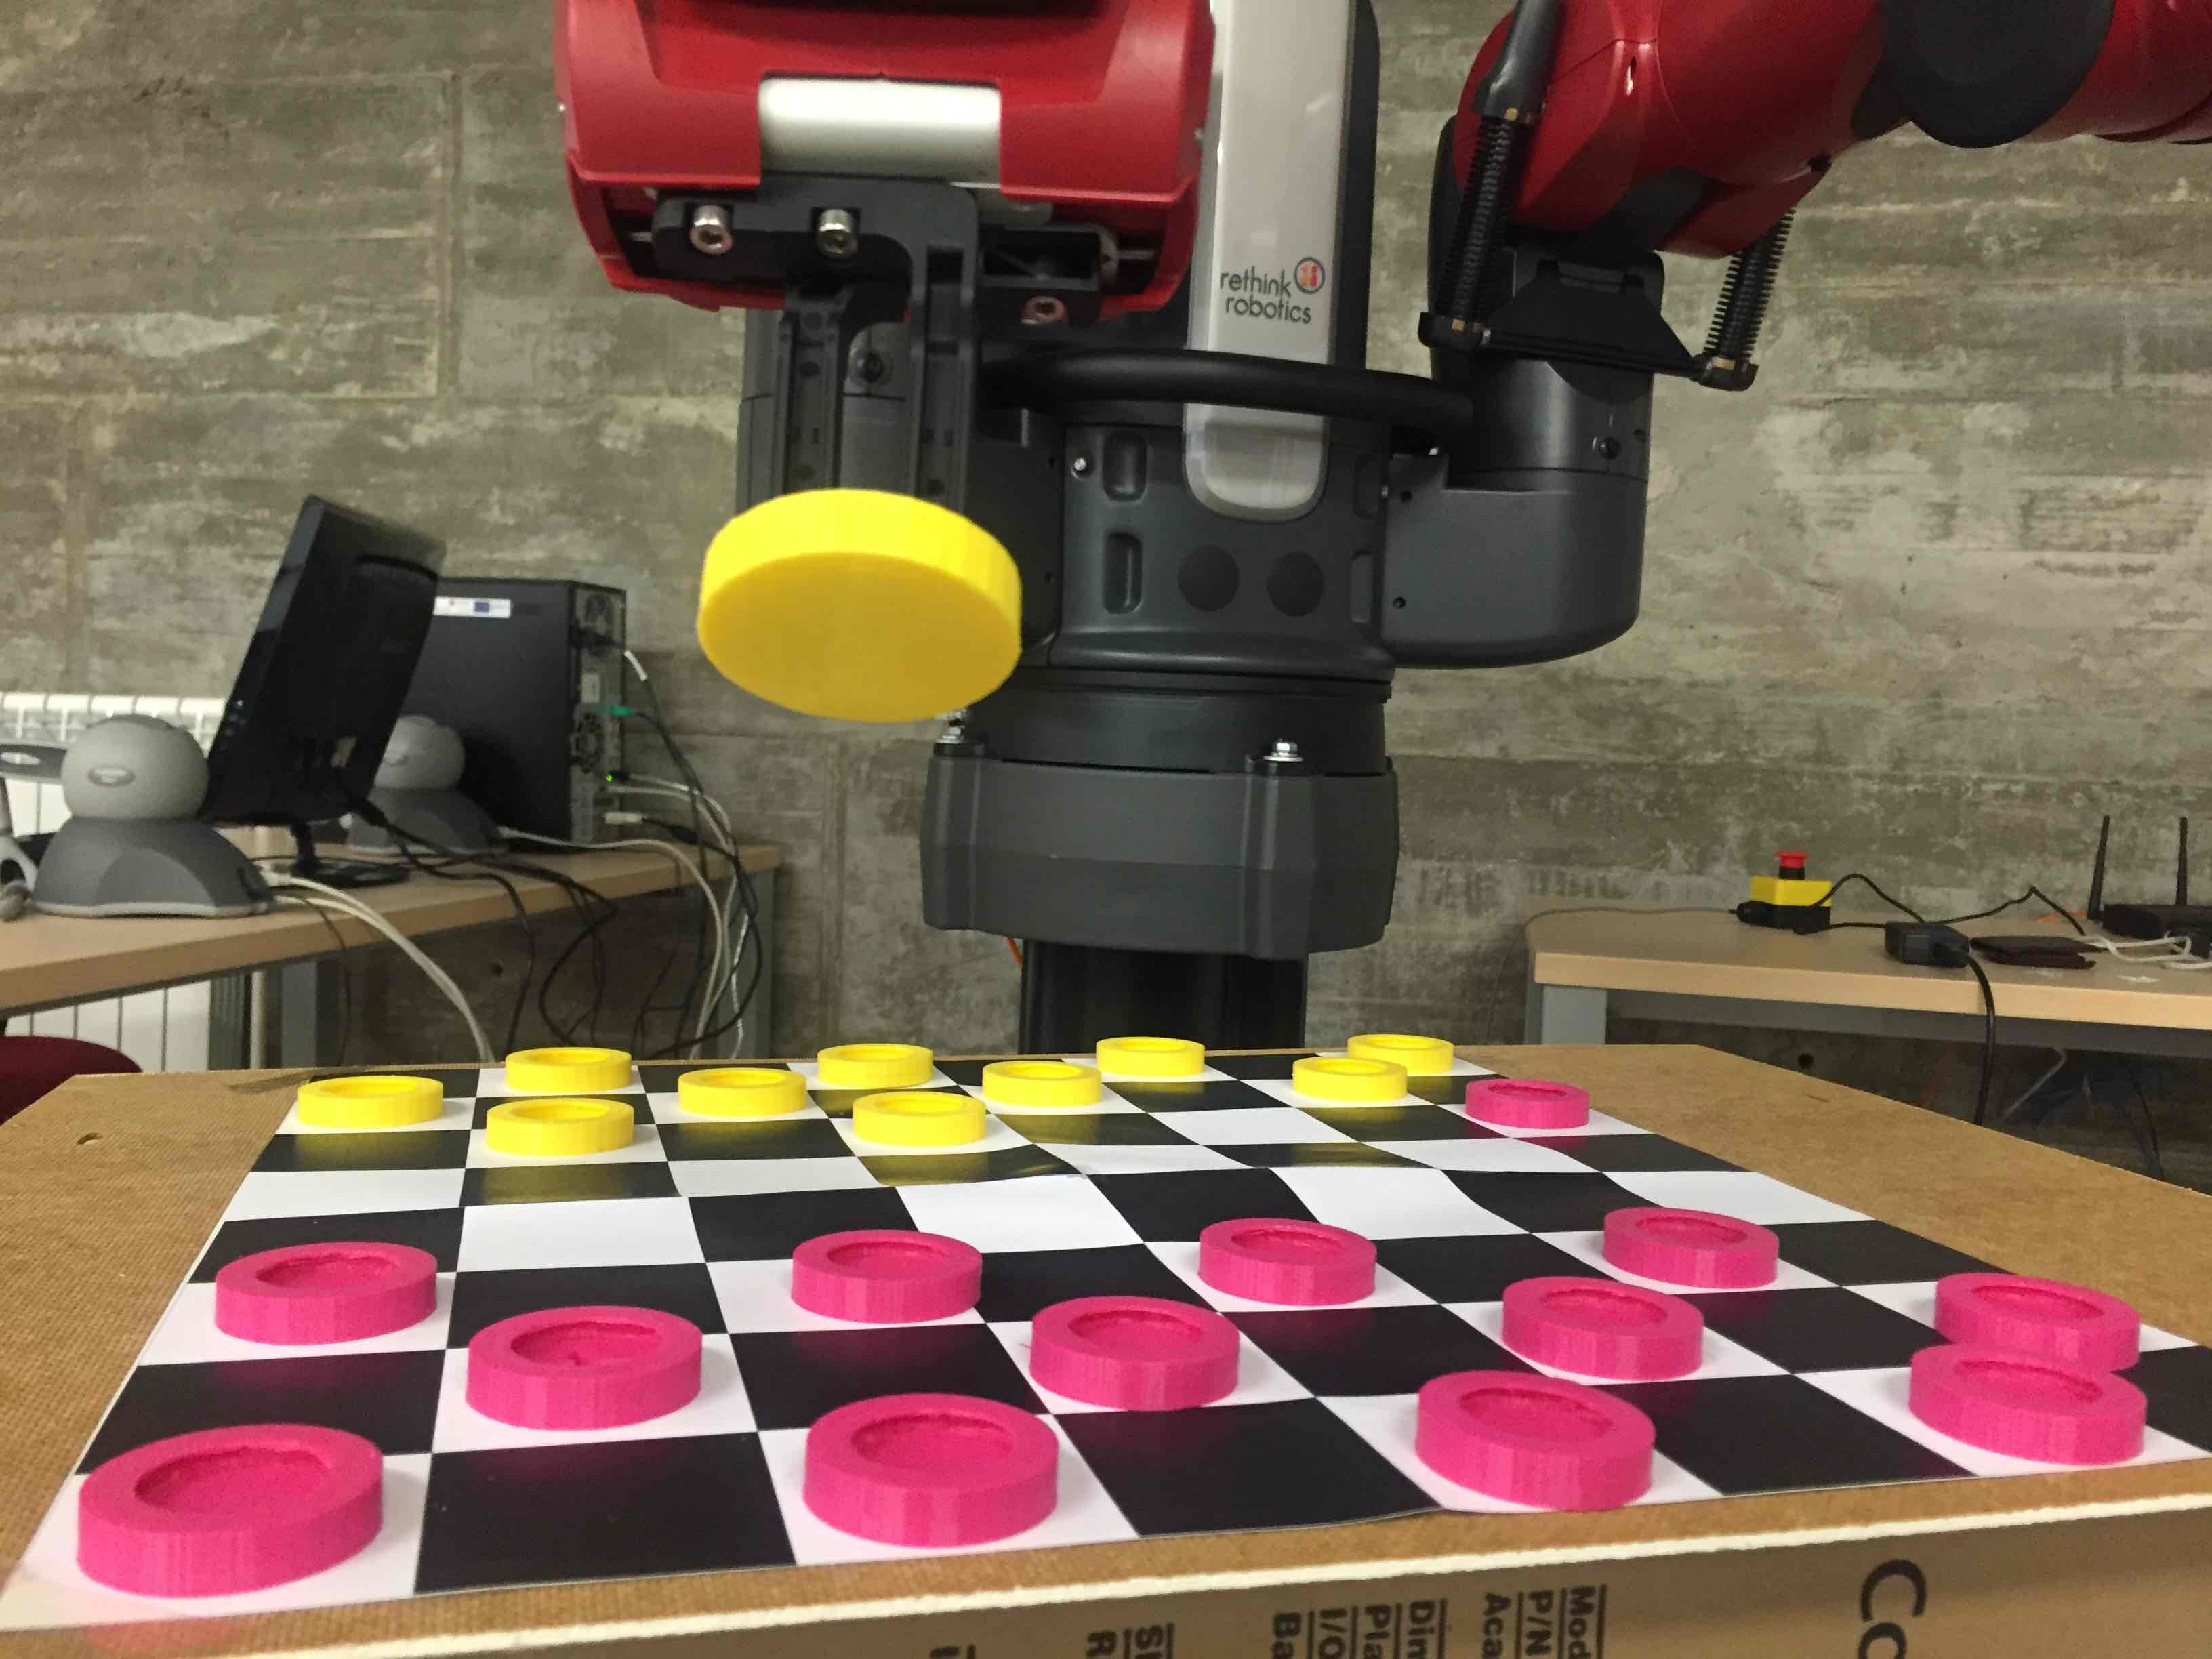
\includegraphics[scale=0.07]{Images/baxterHoldingPiece.jpg} 
%
%
%\begin{table}
%\centering
%\begin{tabular}{c}
%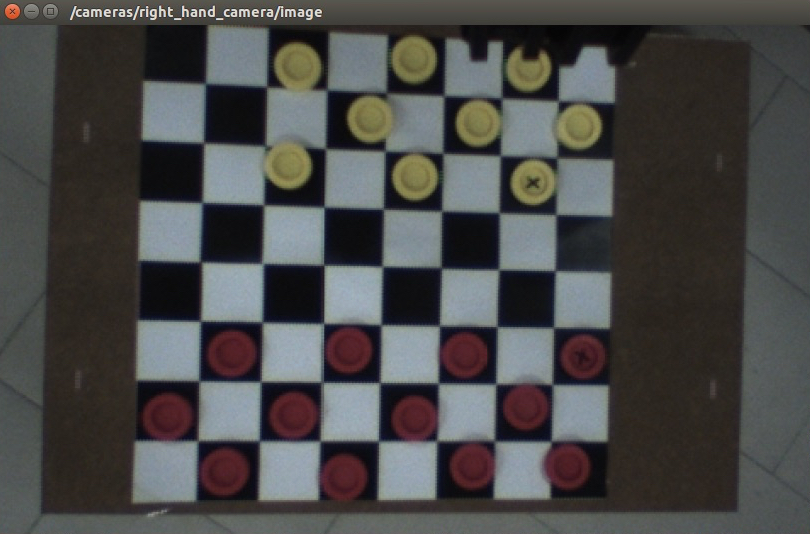
\includegraphics[scale=0.25]{Images/baxterCamaraBrazo.jpg} \\
%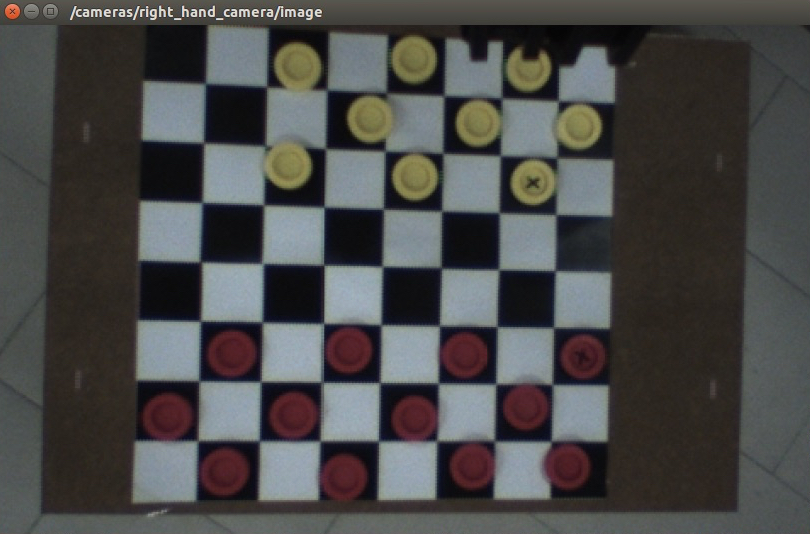
\includegraphics[scale=0.25]{Images/baxterCamaraBrazo.jpg} 
%\end{tabular}
%\caption{\label{tabla_joints} Corresponding joints between robot and haptic device.}
%\end{table}

\begin{table}
\centering
\begin{tabular}{c}
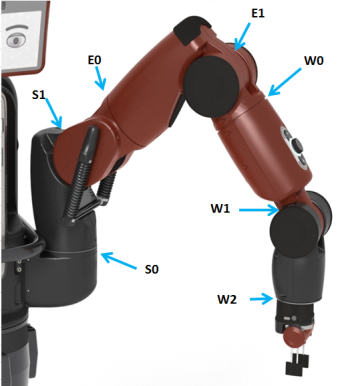
\includegraphics[scale=1.2]{Images/joint_baxter.png} \\
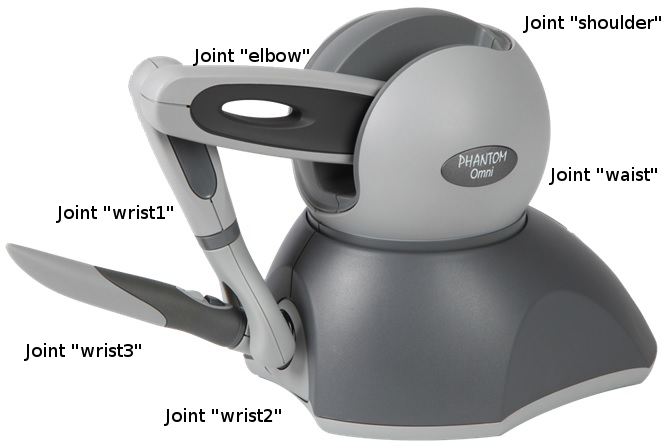
\includegraphics[scale=0.4]{Images/joint_haptico.png} 
\end{tabular}
\caption{\label{tabla_joints} Corresponding joints between robot and haptic device.}
\end{table}

%-Redacción.
%-Archivos.
%-Fotos.
%-Corrección.
%
%Notas :
%	- Mueve un solo brazo (sólo tenemos un háptico)
%	- Sería buena idea revisar las reglas de recogida de datos (impreciso algunas veces)
%	- Revisión correlación de los joints
%	- Ajustar el elbow
%	- Petición para actualizarlo.
%
%-----------------------------------------------------------------------------------------------------------------------------
%Para poder teleoperar a Baxter estamos usando un háptico "Geomatic Touch". 
%Básicamente queremos reproducir los movimientos que realizamos en el háptico en uno de los brazos de Baxter de forma simultánea con el objetivo de poder jugar a las damas.
%
%Primero hemos estudiado los puntos de referencia de Baxter al háptico, ya que al tener menos joints es más complicado transmitir determinados movimientos.
%
%La relación de los joints entre Baxter y el háptico establecida es :
%
%	Baxter		Háptico	
%	S0		"Waist"
%	S1		"Shoulder"
%	E0		No lo usamos
%	E1		"Elbow"
%	W0		No lo usamos
%	W1		"Wrist2"
%	W2		No lo usamos
%
%Estos joints pueden verse en las fotos adjuntas "joint_haptico" y "joint_baxter".
%
%Para poder mover a Baxter con el háptico nos hemos basado en el ejemplo de teleoperación de los brazos por teclado del paquete "Baxter_examples". 
%
%Con ayuda de algunas de las instrucciones que se explican en dicho ejemplo conseguimos que los grippers de Baxter se abran y cierren cuando pulsamos los botones del háptico. (NOTA : PENDIENTE DE REVISIÓN, ya que da problemas recogiendo el brazo)
%
%Después intentamos reproducir los movimientos en el eje X del háptico en Baxter, para luego recoger los ejes Y Z.
%Hemos usado los joints de Baxter S0,S1 y W1 para cada uno de los ejes respectivamente.
%
%------------------------------------------------
%
%Para comunicar los dos nodos (Baxter y Háptico) hacemos que el háptico publique en el topic "geo_touch_right_arm" y en "geo_touch_right_gripper", y que Baxter recoja de los mismos. omni_geo_touch_1
%El háptico solo publica en el topic "geo_touch_right_arm" si uno de los tres joints que usamos se mueve una distancia mayor de 
%|0.01|
%
%También hemos creado un tipo de mensaje personalizado que nos permite comunicar a Baxter qué joint ha de mover y la distancia que ha de moverlo, además de otro que recoge si el gripper debe o no abrirse. 
%Todo ello lo hemos guardado en un paquete "omni_geo_touch_1".
%
%Para ello, en el archivo geo_touch.cpp , hemos ampliado el código para que cuando el háptico se mueva dentro de un determinado rango en un intervalo corto de tiempo (para así evitar movimientos muy leves) publique qué joint tiene que mover Baxter en relación con el que se ha movido en el háptico y la distancia (convertida al rango de Baxter) que debe moverse. 
% 
%------------------------------------------------
%
%Ha sido necesario obtener los valores numéricos de los extremos de cada eje tanto en Baxter como en el háptico.
%Una vez podemos hacer una conversión (cambio de base) apropiada es relativamente sencillo hacer una correlación Háptico-Baxter.
%
%
%Los mayores problemas que hemos tenido han sido ajustar de manera apropiada la distancia de movimiento de los joints en Baxter. El ratio de publicación también ha dado problemas, ya que algunas veces iba muy rápido. 
%A veces, muchos de los movimientos programados quedaban en la cola, con el resultado de que el háptico se movía a la izquierda pero en la cola todavía quedaban mensajes de mover hacia la derecha, produciéndose un retardo notable.





\subsection{Controller}
{\color{red}{Hay que adaptar a nuestro sistema}}

To use this device for the six DOF robot, the robot was broken into two 
sets of three degrees of freedom.  The first system is determined by 
the Cartesian coordinates of the wrist joint.  

The  rotation  of  the  gimbal  is  then  used  to  correspond  to  the  three rotational  degrees  of  freedom  (Rx,  Ry,  and  Rz)  of  the  forearm  of  the  robot.    
By  doing  this,  the  problems  associated  with  multiple  solutions  to  larger  order  degree  of  freedom  robotic  systems  are  mitigated.    
It  is  approximated  that  the  three  axes intersect  at  the  wrist despite the length of the link between the lower arm and forearm.  
This is justified due to the relatively short length of this link and the fact that the robot is controlled based on the vision of a surgeon, allowing for intuitive compensation by the surgeon to position the  end  effector.
This  visual  compensation  is  also  used  to  mitigate  the  effects  of  motor backlash propagation through the robot, although solutions to reduce backlash are being attempted.



\begin{figure*}[ht!]
	\centering
	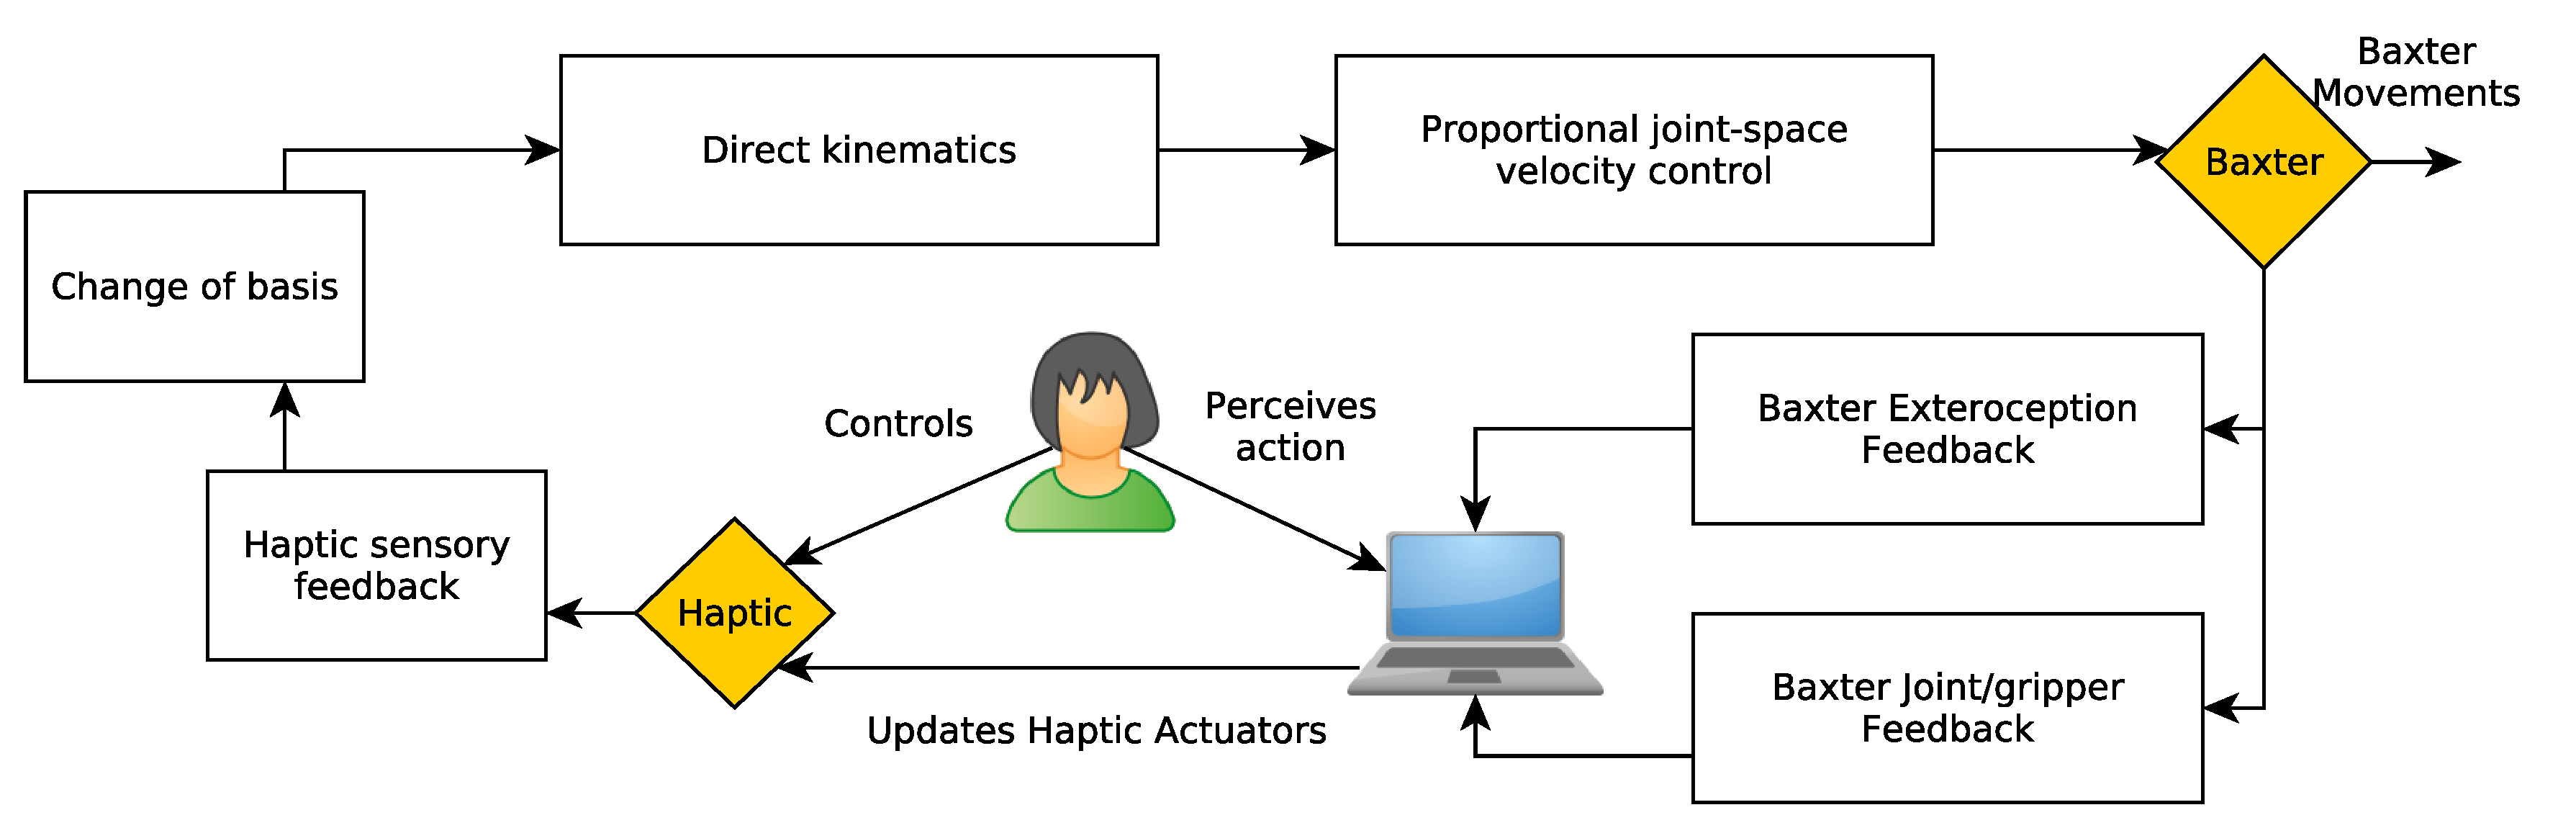
\includegraphics[width=.99\textwidth]{Figures/Controls.pdf} 
	\caption{Haptic-Baxter-Haptic control with human interaction.}
\end{figure*}

\section{Experiment and Results}
\label{sec:experiment}
% SEDANO ? + LAURA Y PABLO?

\subsection{Game description}

Checkers is a strategy gameboard for two players that play on opposite sides of board. It can be played on a 8x8, 10x10 and 12x12 checkerboards.
There are two kind of pieces: the dark pieces and the light pieces. 
The game consists on move a piece diagonally to an adjacent unoccupied square. If the adjacent square contains an opponent's piece, and the square immediately beyond it is vacant, the piece may be captured and take away from the board by jumping over it. During the game each player alternate turns.

\subsection{Board and game pieces adaptation}

To realize our experiment we need to modify the game board, game pieces and the gripper system our robot.
Baxter has two electric parallel grippers that allow our robot to pick up rigid and semi-rigid objects of many shapes and sizes. To play checkers we need that these devices can grab and move game pieces. The shape of these pieces is cylindrical and the height is about three or four milimetres. This requirement makes it difficult for the robot grip firmly the game pieces. Our robot also has two Kits with interchangeable fingers and fingertips to maximize flexibility, and will support customized finger options for specialized parts. We decided to make our own fingers and game pieces to ensure grip and movement of the parts in game development. Figure \ref{3Dprinter} shows the two elements manufactured by a 3D printer.

\begin{figure}[h]
\centering
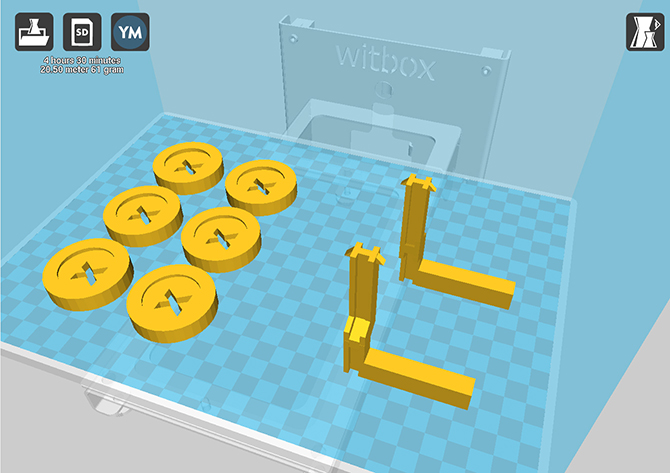
\includegraphics[scale=0.35]{Images/print_3D_2.jpg} 
\caption{\label{3Dprinter}Games pieces and grippers for print in 3D printer.}
\end{figure}

We have also modified the board and we made our own game board where the squares have a size of 55x55 mm, to adapt it to the size of the game pieces (45x45 mm).

After making the changes and to improve the grip of the pieces we have changed the natural way to do that (close the robot grippers) and we do open these grippers.


\subsection{Evaluation}

For evaluation of our experiment we used the Guideline for Ergonomic Haptic Interaction Design (GEHID) developed by L. M. Muñoz, P. Ponsa, and A. Casals \cite{Munoz12}. The guide provides an approach that relates human factors to robotics technology and is based on measures that characterize the haptic interfaces, user’s capabilities and the objects to manipulate. We chose this guide as it is a method that aims to cover aspects of haptic interface design and human-robot interaction in order to improve the design and use of human-robot haptic interfaces in telerobotics applications.

The method to be followed for using the GEDIH guide consists in forming a focus group composed of experts and designers in order to: analyze the indicator, measure the indicator, obtain the GEDIH global evaluation index and finally offer improvement recommendations in the interface design. After the GEDIH validation a user’s experience test can be prepared in order to measure human-robot metrics (task effectiveness, efficiency and satisfaction)~\cite{Andonovski10}.

In a first step we detailed a set of selected indicators that provide a quantitative and/or qualitative measure of the perceived information by the user from the teleoperated environment. In this case we selected the following indicators:
\begin{itemize}
\item \textbf{ReactionForce/Moment}, this indicator measures the variation in the force or moment perceived when contacting with an object or exerting a force over it.
\item \textbf{Pressure}, in this case the variation in the force perceived under a contact with a surface unit it is measured.
\item \textbf{Rigidity}, measure the absence of displacement perceived when a force is exerted. 
\item \textbf{Weight/Inertia}, this indicator measures the resistance that is perceived by user when an object is held statically or is displaced from one place to another.
\item \textbf{Impulse/Collision}, in this case the indicator measures the variation of the linear momentum that happens when colliding with objects in the teleoperated environment.
\item \textbf{Vibration}, this indicator measures the variation in the position perceived when an object is manipulated by user.
\item \textbf{Geometric Properties}, in this case is necessary the perception of the size and shape of the manipulated objects in the teleoperated environment.
\item \textbf{Disposition}, it is also necessary to measure the perception of the position and orientation of objects.
\end{itemize}

In the next stage we identified two different ways of moving the game pieces; one is to drag the tab on the board and another is to raise the piece and move it to the target position. The next step is a tasks allocation for these ways of moving objects. 

In the first case, the sequence of basic task involved are:
\begin{enumerate}
\item Presence. In order to determine if the object is near the grasping tool.
\item Grasping. Is the task that allows the operator to grab an object.
\item Push. Is the task that allows the user to move a game piece by applying a force over it and move it on the board. 
\item Assembling. In order to put the object in the target position.
\item Grasping. In this case to release the object.
\item Presence. In order to release the object.
\end{enumerate}

In the second case, we identified the following basic tasks:
\begin{enumerate}
\item Presence. In order to determine if the object is near the grasping tool.
\item Grasping. Is the task that allows the operator to grab an object.
\item Translating. In order to move the object towards the target place.
\item Assembling. In order to put the object in the target position.
\item Grasping. In this case to release the object.
\item Presence. In order to release the object.
\end{enumerate}

In both cases we observed that previous to the first and last task, the movement of the teleoperated does not requires haptic feedback.

The third step is to establish a clear relationship between selected indicators and basic haptic tasks. Table \ref{indicators} show this relationship. The first column shows the basic tasks involved in our  experiment and the specific indicators are placed in the second column. But also we consider for the design of haptic interface that different tasks have different requirements, both the haptic device as the robot. For example, in the translating task we need game piece weight perception that gives haptic force sensor and grasping force provided by the corresponding robot sensor. Moreover, in our experiment, we use a visual feedback provided by two cameras in the robot to determine the position of the game pieces and the operator can determine the necessary directions and trajectories to perform the desired task. 

\begin{table}[h]
\centering
\caption{\label{indicators}Basic tasks and GEHID indicators.}
\begin{tabular}{ll}
\hline 
\textbf{\footnotesize{}Basic task} & \textbf{\footnotesize{}Indicator}\tabularnewline
\hline 
{\footnotesize{}Presence} & {\footnotesize{}Collision on 3D movement}\tabularnewline
{\footnotesize{}Grasping} & {\footnotesize{}Rigidity on the the grasping tool}\tabularnewline
{\footnotesize{}Push} & {\footnotesize{}Vibration on 3D movement}\tabularnewline
{\footnotesize{}Translating} & {\footnotesize{}Weight on 3D movement}\tabularnewline
{\footnotesize{}Assembling} & {\footnotesize{}Collision on 3D movement}\tabularnewline
\hline 
\end{tabular}

\end{table}

\subsection{User experience}

From the point of view of usability and using as reference the definition provide by the international standard ISO 9241-11 \cite{ISO98} that define usability as “The extent to which a product can be used by specified users to achieve specified goals with effectiveness, efficiency and satisfaction in a specified context of use”, we measure these aspects for our experiment. But we need to include other aspects such as the haptic environment conditions in this classical model approach. L. M. Muñoz, P. Ponsa, and A. Casals \cite{Munoz12} describes in their research a human-robot metric classes that shows table \ref{metric_classes}.

\begin{table}[h]
\centering
\caption{\label{metric_classes}Human-Robot metric classes}
\resizebox{9cm}{!}{
\begin{tabular}{ll} 
\hline 
\textbf{\footnotesize{}Metric classes} & \textbf{\footnotesize{}Description}\tabularnewline
\hline 
{\footnotesize{}Task effectiveness} & {\footnotesize{}Human-robot system performance parameters}\tabularnewline
{\footnotesize{}Automation behaviour efficiency} & {\footnotesize{}Robot behaviour, Interface behaviour}\tabularnewline
{\footnotesize{}Human behaviour efficiency} & {\footnotesize{}Information processing, decision making, action}\tabularnewline
{\footnotesize{}Human behaviour precursors} & {\footnotesize{}Mental workload, fatigue}\tabularnewline
{\footnotesize{}Collaborative metrics} & {\footnotesize{}Human-robot interaction, human-haptic interaction}\tabularnewline
\hline 
\end{tabular}
}
\end{table}

In order to improve the use of our haptic interface we will test the haptic device for a set of expert's evaluators (8 people). We will prepare a user's experience test in order to measured human-robot metrics defined above. We designed a scenario in our usability laboratory in order to apply useful evaluation methods and to improve the human-robot interaction.

\begin{table}[h]
	\centering
	\label{metric_test}
	\caption{Descriptive statistics from Human-Robot experimental results}
%	\resizebox{9cm}{!}{
\begin{tabular}{  l  l }
	\hline
	Description & Result\\ 	\hline
	Subjects& 7\\ 	\hline
	Mean&	77,5329s  \\ 	\hline
	Standard Deviation&	39,1256s  \\	\hline 
	Minimum&	50s\\\hline
	Maximum&	161s\\\hline

\end{tabular}
%}
\end{table}


\begin{figure}[h]
	\centering
	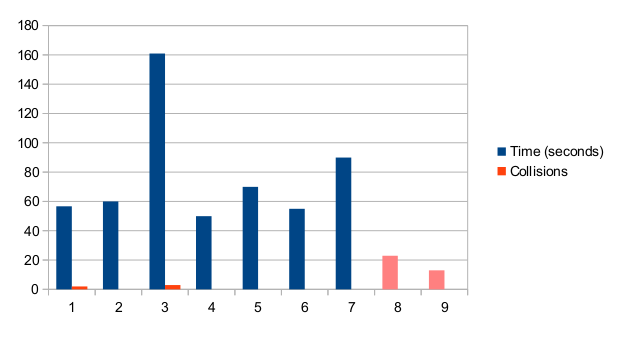
\includegraphics[scale=0.55]{Figures/ResumenDatos_PruebaBasica.png} 
	\caption{\label{3Dprinter}Results overview of experiments performed.}
\end{figure}



\section{Conclusion}
% CAMINO?

The conclusion goes here.


\section*{Acknowledgment}

This work is supported by the \textit{C\'{a}tedra Telef\'{o}nica--Universidad de Le\'{o}n} and it has been partially funded by Spanish \textit{Ministerio de Econom\'{i}a y Competitividad} under grant DPI2013-40534-R.

\begin{thebibliography}{1}

\bibitem{Vertut85}
J.~Vertut and P.~Coiffet, \emph{Teleoperation and Robotics. Applications and Technology}, Spring Netherlands. \hskip 1em plus 0.5em minus 0.4em\relax Vol. 3B, 1985.

\bibitem{Woods04}
D.D.~Woods, J.~Tittle, M.~Feil and A.~Roesler, \emph{Envisioning human-robot coordination in future operations}, IEEE Transactions on Systems, Man and Cybernetics: Part C (Applications and Reviews).\hskip 1em plus 0.5em minus 0.4em\relax Vol. 34, no.2, pp. 210--218, 2004.

\bibitem{Woods97}
D.~Woods and J.~Watts, \emph{How not to have to navigate through too many displays}, In Handbook of Human-Computer Interaction.estricting the field of view: Perceptual
and performance effects.\hskip 1em plus 0.5em minus 0.4em\relax 2nd ed, M.~Helander, T.~Landauer and P~.Prabhu, Eds. Amsterdam, The Netherlands: Elsevier Science, pp. 1177--1201, 1997.

\bibitem{Alfano90}
P.L.~Alfano and G.~F.~Michel, \emph{Restricting the field of view: Perceptual and performance effects}, Perceptual and Motor Skills.\hskip 1em plus 0.5em minus 0.4em\relax Vol. 70, no. 1, pp. 35--45, 1990.

\bibitem{Son13}
H.I.~Son, A.~Franchi, L.L.~Chuang, J.~Kim, H.H.~Bulthoff and P.R.~Giordano, \emph{Human-Centered Design and Evaluation of Haptic Cueing for Teleoperation of Multiple Mobile Robots}, IEEE Transactions on Systems, Man and Cybernetics: Part B (Cybernetics).\hskip 1em plus 0.5em minus 0.4em\relax Vol. 43, no. 2, pp. 597--609, 2013.

\bibitem{Sitti03}
M.~Sitti and H.~Hashimoto, \emph{Teleoperated Touch Feedback From the Surfaces at the Nanoscale: Modeling and Experiments}, IEEE ASME Transactions on Mechatronics.\hskip 1em plus 0.5em minus 0.4em\relax Vol. 8, no. 2, pp. 287--298, 2003.

\bibitem{Diolaiti02}
N.~Diolaiti and C.~Melchiorri, \emph{Tele-Operation of a Mobile Robot Through Haptic Feedback}, In Proceedings of the IEEE International Workshop on Haptic Virtual Environments and Their Applications (HAVE 2002).\hskip 1em plus 0.5em minus 0.4em\relax, Ottawa, Ontario, Canada, 17-18 November, 2002.

\bibitem{King09}
C.H.~King, M.O.~Culjat, M.L.~Franco, C.E.~Lewis, E.P.~Dutson, W.S.~Grundfest and J.W.~Bisley, \emph{Tactile Feedback Induces Reduced Grasping Force in Robot-Assisted Surgery}, IEEE Transactions on Haptics.\hskip 1em plus 0.5em minus 0.4em\relax Vol. 2, no. 2, pp. 103--110, 2009.

\bibitem{Kron04}
A.~Kron, G.~Schmidt, B.~Petzold, M.I.~Zah, P.~Hinterseer and E.~Steinbach, \emph{Disposal of explosive ordnances by use of a bimanual haptic telepresence system}, In Proceedings of the IEEE International Conference on Robotics and Automation (ICRA 04).\hskip 1em plus 0.5em minus 0.4em\relax pp. 1968--1973, 2004.

\bibitem{SuarezRuiz12}
%TODO aplicar estilo adecuado a esta referencia
F.~Suarez-Ruiz, \emph{phantom-omni}, {https://github.com/fsuarez6/phantom\_{}omni}

\bibitem{Munoz12}
L.M.~Mu{\~{n}}oz, P.~Ponsa and A.~Casals, \emph{Design and Development of a Guideline for Ergonomic Haptic Interaction}, In Human-Computer Systems Interaction: Backgrounds and Applications 2: Part 2, Z.~Hippe and J.L.~Kulikowski and T.~Mroczek, Eds. Springer Berlin Heidelberg, pp. 15--19, 2012.

\bibitem{Andonovski10}
B.~Andonovski, P.~Ponsa and A.~Casals, \emph{Towards the development of a haptics guideline in human-robot systems}, Human System Interactions (HSI), 2010 3rd Conference on, Rzeszow, pp. 380--387, 2010.

\bibitem{ISO98}
ISO, \emph{ISO 9241-11:1998 Ergonomic requirements for office work with visual
display terminals (VDTs) – part 11: Guidance on usability}, 1998.


\end{thebibliography}
\end{document}


